%! TeX program = lualatex
\documentclass[../main.tex]{subfiles}
\begin{document} \section{Introduction to mathematical models (of biological processes)}

As a scientist, we observe nature and try to create reasonable predictions of the physical world. Scientific theory describes the real world using models. Here are some models we are most like to be familiar with.

\begin{enumerate}
  \item The solar system \url{https://eyes.nasa.gov/apps/solar-system/}
  \item Newton's \(F = ma\).
  \item The law of supply and demand in economics.
\end{enumerate}

Let's learn to ask basic questions about models (instead of taking them for granted because they are discovered by some famous person).
\begin{enumerate}[wide]
  \item Do they accurate in every possible way? 

    \todo{leads to the discussion of making assumptions.}
    \blanklines{5}

  \item Do they make sense? 

    \todo{leads to the discussion of everyday experience and dimensional homogeneity.}
    \blanklines{5}

  \item Are they provide knowledge and insights? 

    \todo{for fun and general interests.}
    \blanklines{5}

  \item Are they relatively easy to work with? 

    \todo{The purpose of this question is to project openness (from the instructor). The answer should be ``that depends, but different skills lead to different opportunities.''}
    \blanklines{5}
\end{enumerate}

\clearpage
\vspace{-1in}
\centerline{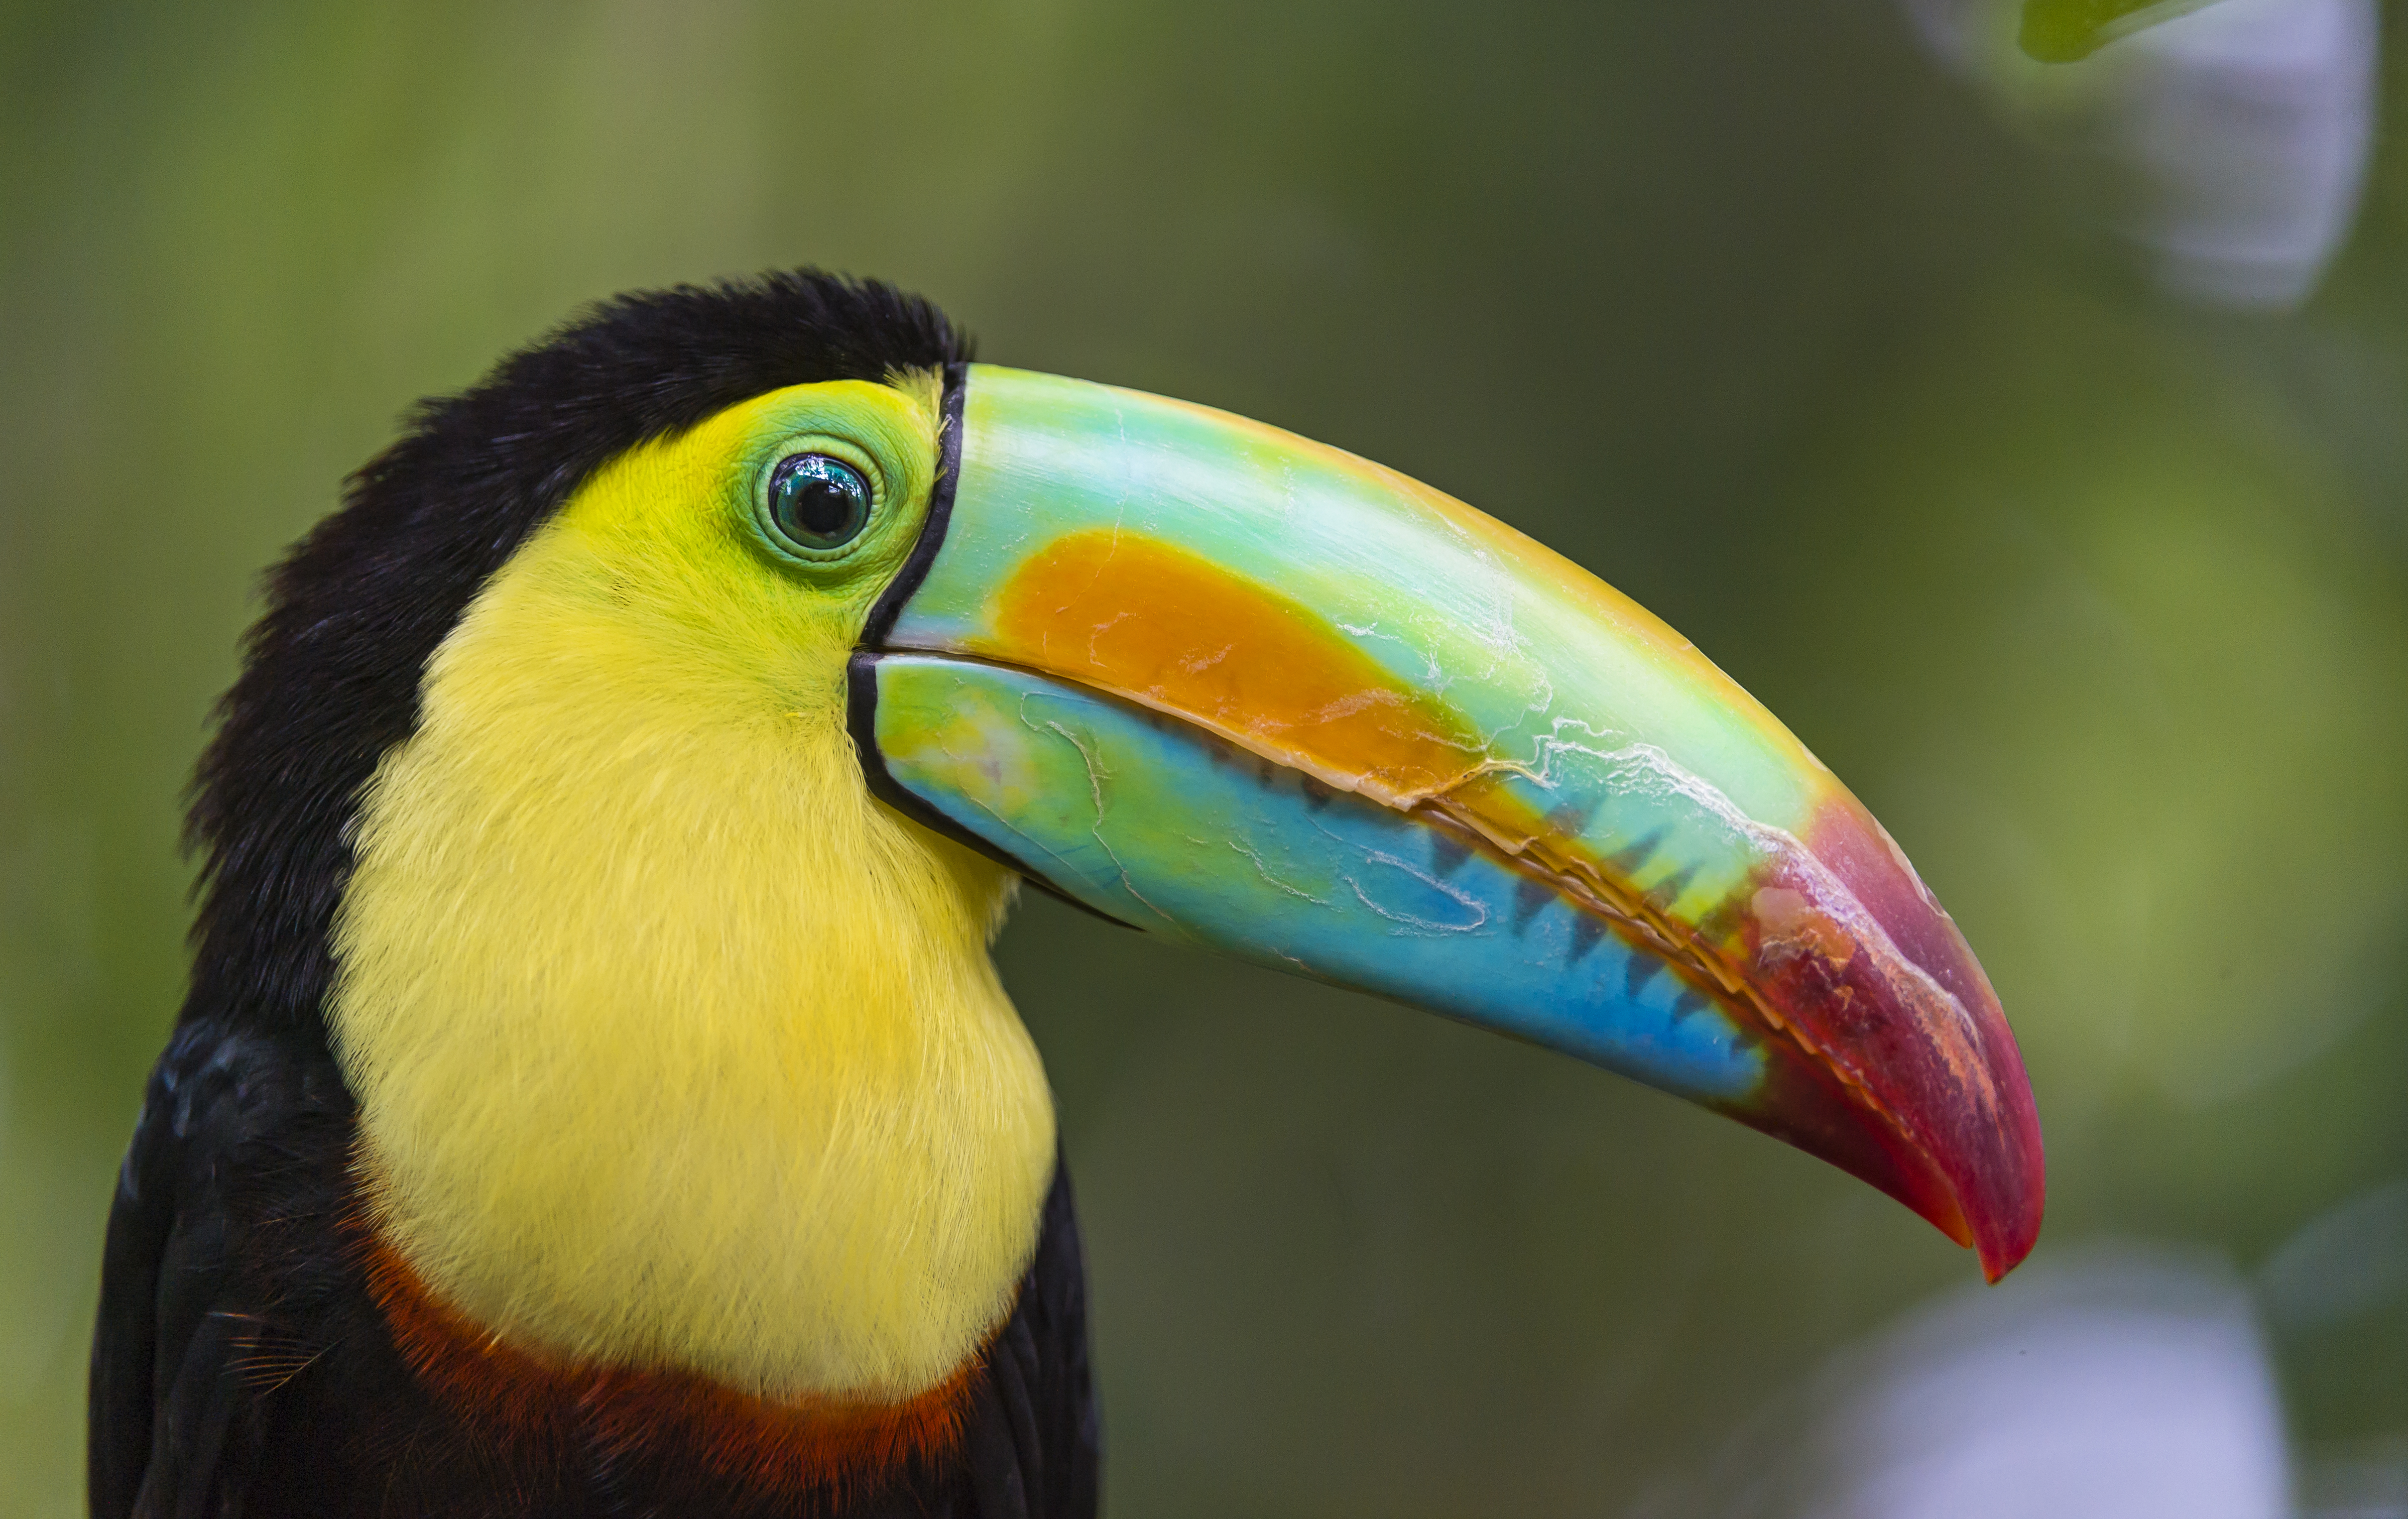
\includegraphics[width=\pagewidth]{../standalones/image-toucan}}
\todo{TODO: Replace this random image found on the internet.}

\begin{example}[Birds of Costa Rica] \label{ex:toucan}
  An ecologist studies birds in rain forests. After a visit to Costa Rica, they bring back data relating the size of a bird to their weight. However, the ecologist does not have data on the beautiful toucan and is now \emph{invested} in the following question.

  \begin{center}
    \hlmain{How much does an adult toucan weigh given that it measures roughly 40 cm in length?}
  \end{center}

  We represent weight by \(w\) and length by \(\ell\). Two interns put forth their analysis. 
  \begin{description}[wide]
    \item[Intern A.] A cubic curve \(w = 0.006 \ell^{3}\) seems to fit the data really well.
    \item[Intern B.] A quadratic curve \(w = 0.25 \ell^{2}\) seems to work just as well.
  \end{description}

  Interestingly, both interns' arguments lead to \emph{remarkably similar} predictions that an adult toucan should weight about 400g. \hlmain{\faComment{} You are the ecologist. How do you evaluate your interns' arguments?}

  \includegraphics{../standalones/build/plot-birds-of-costa-rica-arg1}
  \includegraphics{../standalones/build/plot-birds-of-costa-rica-arg2}

  \todo{Note: 10 minutes group work. End with an iClicker poll.}

  \begin{enumerate}[wide]
    \item Which equation make more physical sense? Recall that \(\text{weight} = (\text{density}) \times (\text{volume})\). 
      \blanklines{10}

    \item Which equation fits the data better? 

      It is really hard to visually tell which intern's curve fit the data better. However, because they are both polynomial equations, we can apply the log-log transformation. More on the theory later. For now, let's focus on the result.

      \todo{Note: I deviate from Geoff's note and plot a log-log transformation of length against weight. The slope \(n\) of the best-fit line is the exponent in the desired model \(w = k \ell^{n}\).}

      \begin{center}
        \includegraphics{../standalones/build/plot-birds-of-costa-rica}
        \quad
        \includegraphics{../standalones/build/plot-birds-of-costa-rica-loglog}
      \end{center}

      It seems unquestionable that a \underline{\hspace{3in}} fits the transformed data well. What does that mean?  The line in log-log space should have the form
      \blanklines{3}
      It follows that 
      \blanklines{5}

  \end{enumerate}
\end{example}
\end{document}
